% !TeX spellcheck = ru_RU-Russian
% !TeX program = xelatex
% !BIB TS-program = biber

\documentclass{beamer}

\usepackage[utf8]{inputenc}
\usepackage[russian]{babel}

%---tikz----
\usepackage{tikz}
\usetikzlibrary{arrows, chains, matrix, positioning, scopes, patterns, shapes}
\usepackage{pgfplots, subfigure}
\usepackage{ulem}

%\usepackage[backend=biber,firstinits=true,hyperref=true,style=numeric-comp]{biblatex}

\usepackage{../beamerthemeec2020}
%{\footnotesize\bibliography{../biblio}}

\title{Эллиптические кривые}
\subtitle{Лекция 1. Введение}
\author{Семён Новосёлов}
\institute{БФУ им. И. Канта}
\date{2025}

\begin{document}
    

\frame{\titlepage}

\begin{frame}{Мотивация}
    \structure{Криптография:}

    \begin{itemize}
        \item классическая -- дискретный логарифм (ECDH, ECDSA)
        \item постквантовая -- схемы на изогениях (CSIDH, SQISign)
    \end{itemize}
    
    \vspace{1em}
    
    База для построения множества схем и протоколов.
\end{frame}

\begin{frame}{Примеры использования}
Классическая криптография в реальном мире:
\vspace{0.5em}
\begin{itemize}
	\item \structure{https} (TLS): цифровая подпись
	\item \structure{WireGuard VPN} в составе ядра Linux:
	\\Curve25519, обмен ключами
	\item \structure{SSH}: кривая Эдвардса Ed25519
	\item \structure{Bitcoin/Ethereum}: кривая Secp256k1, цифровая подпись
\end{itemize}
\end{frame}

\begin{frame}{Пример. TLS}
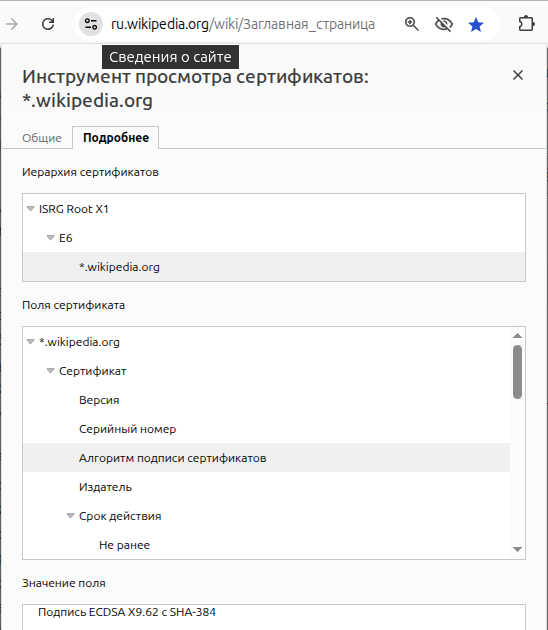
\includegraphics[scale=0.35]{../images/example_tls}
\end{frame}

\begin{frame}{Постквантовая криптография: перспективы}
	Полный \structure{отказ} от классической криптографии (\structure{ECDSA}, \structure{ECDH}, \structure{FFDH}, \structure{RSA}) рекомендован NIST начиная с \structure{2035}\footnote{\url{https://csrc.nist.gov/csrc/media/Presentations/2025/nist-pqc-the-road-ahead/images-media/rwcpqc-march2025-moody.pdf}}.
	
	\vspace{0.5em}
	А с \structure{2030} классические схемы объявлены \structure{устаревшими}.
	
	\vspace{0.5em}
	
	Замена для эллиптических кривых:
	\begin{itemize}
		\item цифровые подписи: \structure{ECDSA} \structure{$\rightarrow$} \structure{SQISign}
		\item обмен ключами: \structure{ECDH} \structure{$\rightarrow$} \structure{CSIDH}
	\end{itemize}
%\structure{SIKE/SIDH}: обмен ключами
%\begin{itemize}
%    \item был кандидатом на стандартизацию в Round 3 NIST
%    \begin{tcolorbox}[colframe=title-and-section-color!120, colback=title-and-section-color!5, title=SIKE Cryptographic Challenge, center title]
%    	\begin{itemize}
%    		\item {\small
%    			\href{https://github.com/microsoft/SIKE-challenges/}{github.com/microsoft/SIKE-challenges/}}
%    		\item 5000 USD или 50 000 USD за взлом
%    	\end{itemize}
%    \end{tcolorbox}
%    \item взломан Castryck и Decru, используя информацию о точках кручения в протоколе
%    \item замена: \structure{weakSIDH}, \structure{CSIDH}
%\end{itemize}

%\vspace{0.5em}
%Есть также подписи: \structure{OSIDH}, \structure{SQISign}.
%\vspace{0.5em}
%\begin{scriptsize}
%	\begin{itemize}
%		\item[\structure{*}] Castryck W., Decru T. An efficient key recovery attack on SIDH. \url{https://eprint.iacr.org/2022/975}
%		\item[\structure{*}] \url{https://issikebrokenyet.github.io/}
%	\end{itemize}
%\end{scriptsize}

\vspace{0.5em}
\structure{!} В настоящее время схемы на изогениях не утверждены в качестве стандартов.
\end{frame}

\begin{frame}{План курса}
\begin{enumerate}
    \item Введение
    \item Групповой закон на эллиптической кривой
    \item Точки $n$-кручения
    \item Алгоритмы подсчета $\mathbb{F}_q$-рациональных точек кривой
    \item Алгоритм факторизации на эллиптических кривых
    \item Тест на простоту Goldwasser-Kilian
    \item Выбор эллиптической кривой для криптографии
    \item Криптографические схемы на изогениях
\end{enumerate}
\end{frame}

\begin{frame}{Порядок работы}
	\structure{Формат:} лекции \structure{+} сдача лабораторных работ
\vspace{0.5em}
\begin{itemize}
	\item после лекций выкладываются лабораторные работы
	\item срок сдачи: \structure{2} недели
	\item за пределами срока сдачи работы принимаются с низким приоритетом и в количестве не более \structure{2} за пару
\end{itemize}
\vspace{0.5em}
\structure{Экзамен}: сдать \structure{85\%} лабораторных и \structure{курсовую}
\begin{itemize}
	\item оценка -- среднее по оценкам за сдачу лабораторных
\end{itemize}
\end{frame}

\begin{frame}{Определение}
	Уравнение Вейерштрасса \structure{в аффинных координатах}:
	\begin{equation}\label{eq:weierstrassequation}
		f: y^2+a_1xy + a_3y = x^3 + a_2x^2 + a_4x + a_6
	\end{equation}

	Уравнение над полем~$K$ -- \structure{гладкое}, если во множестве его решений над~$\overline{K}$ нет сингулярных точек.
	\vspace{1em}
	
	\structure{Эллиптическая кривая} задаётся как \[E(K) = \{ (x,y) \in K \times K: f(x,y)=0 \} \cup \{\mathcal{O}\}
	\]
	для гладкого~$f$.
	\begin{itemize}
		\item $\mathcal{O}$ -- точка в бесконечности.
		\item $K$ -- некоторое поле, чаще всего $K = \mathbb{F}_q$.
	\end{itemize}
\end{frame}


\begin{frame}{Проективные координаты}
    %\structure{Обозначения.}
    %$\mathbb{F}_q$ -- конечное поле, $|\mathbb{F}_q| = q = p^n$, $K$ -- поле, $\overline{K}$ -- алг. замыкание.
    
    \structure{Уравнение Вейерштрасса} в проективных координатах: 
        \begin{equation}
            \label{eq:weierstrass}
            F: Y^2Z + a_1 X Y Z + a_3 Y Z^2 = X^3 + a_2 X^2 Z + a_4 X Z^2 + a_6 Z^3,
        \end{equation}
        где $a_i \in K$.
        \begin{itemize}
            %\item \structure{гладкое} (или несингулярное): $\forall P \in \mathbb{P}^2(K)$, $\frac{dF}{dX}(P) \neq 0$, $\frac{dF}{dY}(P) \neq 0$ или $\frac{dF}{dZ}(P) \neq 0$.
            \item \textcolor{struct-color}{сингулярное}: $\exists P \in \mathbb{P}^2(K): \frac{dF}{dX}(P) = \frac{dF}{dY}(P) = \frac{dF}{dZ}(P) = 0$.
            \item  \textcolor{struct-color}{гладкое} (или несингулярное) в противном случае.
        \end{itemize}
        %\footnotetext[1]{проективная плоскость над $K$ — множество классов эквивалентности на $K^3\setminus \{0,0,0\}$, т.е. $\overrightarrow{X} \sim \overrightarrow{Y}$, если $x_1=u*y_1,x_2=u*y_2,x_3=u*y_3$ }
    %\structure{Эллиптическая кривая}:
    
    \vspace{1em}
    
    \structure{Эллиптическая кривая $E$} -- множество точек $\mathbb{P}^2(K)$, удовлетворяющих гладкой кривой \eqref{eq:weierstrass}.
        
    \begin{itemize}
        \item Точка в бесконечности: $\exists! \mathcal{O} = (0: 1: 0)$.
    \end{itemize}

	\begin{itemize}
	\item Проективные координаты позволяют избежать деления в арифметике за счёт доп. умножений.
\end{itemize}
\end{frame}

\begin{frame}{Дискриминант}
    Как проверить, что уравнение Вейерштрасса задаёт эллиптическую кривую? Обозначим
    \begin{equation}
        \begin{split}
            d_2 &= a_1^2 + 4a_2 \\
            d_4 &= 2a_4 + a_1a_3 \\
            d_6 &= a_3^2 + 4a_6 \\
            d_8 &= a_1^2a_6 + 4a_2a_6 - a_1a_3a_4 + a_2a_3^2 - a_4^2 \\
            c_4 &= d_2^2 - 24d_4 \\
            %\text{Для проверки: } 4d_8 &= d_2d_6 - d_4^2
        \end{split}
    \end{equation}
    Тогда \structure{дискриминант} уравнения \eqref{eq:weierstrassequation} определяется как 
    \[
    \Delta = -d_2^2d_8 - 8d_4^3-27d_6^2+9d_2d_4d_6.
    \]
\end{frame}


\begin{frame}{Классификация уравнений Вейерштрасса}
    \begin{tcolorbox}[colframe=title-and-section-color!120, colback=title-and-section-color!5, title=Теорема \text{[Silverman, Thm. 1.4]}, center title]
        \begin{enumerate}
            \item $\Delta \neq 0 \iff$ кривая гладкая ($\implies$ задаёт эллиптическую кривую) 
            \item $\Delta = 0, c_4 \neq 0 \iff$ кривая обладает узлом (node) 
            \item $\Delta = c_4 = 0 \iff$ кривая обладает точкой перегиба (cusp)
        \end{enumerate}
    \end{tcolorbox}
\end{frame}

\begin{frame}{Классификация уравнений Вейерштрасса - $2$}
             \begin{block}{$\Delta < 0$}
                  \begin{figure}[h!]
                      \begin{tikzpicture}
                         \begin{axis}[
                             xmin=-5,
                             xmax=5,
                             ymin=-7,
                             ymax=7,
                             xlabel={$x$},
                             ylabel={$y$},
                             scale only axis,
                             axis lines=middle,
                             domain=-2.1038:3,
                             samples=200,
                             smooth,
                             clip=false,
                             axis equal image=true,
                             ]
                             \addplot [red] {sqrt(x^3-3*x+3)}
                             node[right] {$y^2=x^3-3x+3$};
                             \addplot [red] {-sqrt(x^3-3*x+3)};
                         \end{axis}
                     \end{tikzpicture} 
                \end{figure} 
            \end{block}
\end{frame}

\begin{frame}{Классификация уравнений Вейерштрасса - $3$}
      \begin{block}{$\Delta > 0$}
        \begin{figure}[h!]
            \centering
            \begin{tikzpicture}
                \begin{axis}[
                    xmin=-1.5,
                    xmax=1.5,
                    ymin=-2,
                    ymax=2,
                    xlabel={$x$},
                    ylabel={$y$},
                    scale only axis,
                    axis lines=middle,
                    domain=-1:0, 
                    samples=200,
                    smooth,
                    clip=false,
                    axis equal image=true,
                    ]
                    \addplot [red] {sqrt(x^3-x)};
                    \addplot [red] {-sqrt(x^3-x)};
                \end{axis}
                \begin{axis}[
                    xmin=-1.5,
                    xmax=1.5,
                    ymin=-2,
                    ymax=2,
                    xlabel={$x$},
                    ylabel={$y$},
                    scale only axis,
                    axis lines=middle,
                    domain=0.1:1.5, 
                    samples=200,
                    smooth,
                    clip=false,
                    axis equal image=true,
                    ]
                    \addplot [red] {sqrt(x^3-x)}
                    node[right] {$y^2=x^3-x$};
                    \addplot [red] {-sqrt(x^3-x)};
                \end{axis}
            \end{tikzpicture}
        \end{figure}
    \end{block}
\end{frame}

\begin{frame}{Изоморфизмы эллиптических кривых}
Пусть $E_1/K, E_2/K$ -- эллиптические кривые с уравнениями:
\begin{equation}
\begin{split}
E_1&: y^2+a_1xy + a_3y = x^3 + a_2x^2 + a_4x + a_6 \\
E_2&: y^2+a_1'xy + a_3'y = x^3 + a_2'x^2 + a_4'x + a_6'
\end{split}
\end{equation}
    
$E_1/K, E_2/K$ \structure{изоморфны}, если они изоморфны как проективные многообразия.%, т.е. $\exists$ морфизмы $\phi: E_1/K \to E_2/K, \psi: E_2/K \to E_1/K$ (определённые над $K$), такие что $\psi \circ \phi = id_{E_1}, \phi \circ \psi = id_{E_2}$.

\begin{tcolorbox}[colframe=title-and-section-color!120, colback=title-and-section-color!5, title=Теорема, center title]
$E_1 \simeq E_2 \iff \exists u,r,s,t \in K, u \neq 0$ такие, что замена
\begin{equation}
    \label{eq:isom}
    (x,y) \mapsto (u^2x+r, u^3y+ u^2sx+t)
\end{equation}
преобразует кривую $E_1$ в $E_2$.
\end{tcolorbox}

Изоморфизм кривых задаёт отношение эквивалентности.
\end{frame}

\begin{frame}{Изоморфизмы -- зачем нужно?}
    Позволяют подбирать форму кривой под нужные свойства в арифметике. Например:
    \begin{itemize}
        \item с меньшим кол-вом коэффициентов: ускорение вычислений 
        \item с константным временем выполнения группового закона: противодействие атакам по побочным каналам
    \end{itemize}
\end{frame}

\begin{frame}{Краткие формы}
    \begin{equation*}
        E/K: y^2 + a_1 xy + a_3 y = x^3 + a_2 x^2 + a_4 x + a_6 \tag{\ref{eq:weierstrassequation}}
    \end{equation*}
    \structure{$\operatorname{char} K \neq 2$:}
    Изоморфизм \[(x, y)\mapsto \left(x, \frac{1}{2}(y-a_1x-a_3)\right)\] преобразует $E/K$ к виду:
    \begin{equation}
        \label{eq:char_neq2}
        E/K: y^2 = 4x^3 + d_2x^2 + 2d_4 + d_6.
    \end{equation}
    
    \structure{$\operatorname{char} K \neq 2, 3$:}
    Изоморфизм
    \[
    (x, y) \mapsto \left(\frac{x-3d_2}{36}, \frac{y}{216}\right)
    \]
    Преобразует~\eqref{eq:char_neq2} к виду:
    \begin{align}
        E/K: y^2 = x^3 + ax + b
    \end{align}
    \[
    a = -27 c_4
    \]
    \[
    b = -56(d_2^3 + 36 d_2 d_4 - 216 d_6) 
    \]
\end{frame}

\begin{frame}{Краткие формы - $2$}
В последнем случае, 
\begin{align*}
    \Delta &= -16(4a^3 + 27b^2) \\ \nonumber
\end{align*}
\structure{$char K = 2$:} 
\[
a_1 \neq 0 \implies (x, y) \mapsto \left(a_1^2x+\frac{a_3}{a_1}; \, a_1^3y + \frac{a_1^2a_4+a_3^2}{a_1^3}\right)
\]
\begin{equation}
    E/K: y^2+xy=x^3+a_2'x^2+a_6'
\end{equation}

\[
a_1 \neq 0 \implies (x, y) \mapsto (x+a_2, y)
\]
\begin{equation}
    E/K: y^2+a_3y = x^3+a_4x+a_6
\end{equation}
\end{frame}

\begin{frame}{Определение изоморфности кривых}
\structure{$j$-инвариант} эллиптической кривой $E$:
\[
j(E) = \frac{c_4^3}{\Delta}
\] или для краткой формы  $j(E) = -1728 \frac{4a^3}{\Delta}$.
\begin{center}
    \begin{tcolorbox}[enhanced,hbox,colback=title-and-section-color!5,colframe=title-and-section-color!120,title=Теорема,center title]
        \begin{varwidth}{\textwidth}
            \begin{center}
                $E_1 \simeq E_2$ над $\overline{K} \iff j(E_1)=j(E_2)$
            \end{center}
        \end{varwidth}
    \end{tcolorbox}	
\end{center}
Определение изоморфности кривых над полем $K$: проверка условий теоремы. Если выполняется -- составление и решение системы уравнений используя \eqref{eq:isom}.
\end{frame}

\begin{frame}{Литература}
\begin{enumerate}
    \item Washington L.C. "Elliptic curves number theory and cryptography"%. 2ed (2008)
    \item Menezes A. "Elliptic curve public key cryptosystems"
    \item Hankerson D., Menezes A., Vanstone S. "Guide to elliptic curve cryptography"
    \item Blake I., Seroussi G., Smart N. "Elliptic Curves in Cryptography"
    \item Silverman J.H. "The Arithmetic of Elliptic Curves"%, 2ed (2009)
\end{enumerate}

%\nocite{Blake1999}
%\printbibliography

\begin{center}
    \begin{tcolorbox}[enhanced,hbox,colback=block-green-color-bg,colframe=subsection-color!120,title=Контакты,center title]
        \begin{varwidth}{\textwidth}
            \begin{center}
                \href{mailto:snovoselov@kantiana.ru}{snovoselov@kantiana.ru}
            \end{center}
        \end{varwidth}
    \end{tcolorbox}	
\end{center}

\structure{Страница курса:}\\
{\footnotesize
    \href{https://crypto-kantiana.com/semyon.novoselov/teaching/elliptic_curves_2025}{crypto-kantiana.com/semyon.novoselov/teaching/elliptic\_curves\_2025}
}
\end{frame}

\begin{frame}{Темы курсовых}
	\begin{enumerate}
		\item Криптоанализ схем на изогениях (несколько тем)
		\item Схема цифровой подписи SQISign
		\item Атака Кастрика-Декру
		\item \href{https://crypto-kantiana.com/thesis_topics.html}{crypto-kantiana.com/thesis\_topics.html}
	\end{enumerate}
\end{frame}

\end{document}
